% Options for packages loaded elsewhere
\PassOptionsToPackage{unicode}{hyperref}
\PassOptionsToPackage{hyphens}{url}
%
\documentclass[
]{article}
\usepackage{amsmath,amssymb}
\usepackage{iftex}
\ifPDFTeX
  \usepackage[T1]{fontenc}
  \usepackage[utf8]{inputenc}
  \usepackage{textcomp} % provide euro and other symbols
\else % if luatex or xetex
  \usepackage{unicode-math} % this also loads fontspec
  \defaultfontfeatures{Scale=MatchLowercase}
  \defaultfontfeatures[\rmfamily]{Ligatures=TeX,Scale=1}
\fi
\usepackage{lmodern}
\ifPDFTeX\else
  % xetex/luatex font selection
\fi
% Use upquote if available, for straight quotes in verbatim environments
\IfFileExists{upquote.sty}{\usepackage{upquote}}{}
\IfFileExists{microtype.sty}{% use microtype if available
  \usepackage[]{microtype}
  \UseMicrotypeSet[protrusion]{basicmath} % disable protrusion for tt fonts
}{}
\makeatletter
\@ifundefined{KOMAClassName}{% if non-KOMA class
  \IfFileExists{parskip.sty}{%
    \usepackage{parskip}
  }{% else
    \setlength{\parindent}{0pt}
    \setlength{\parskip}{6pt plus 2pt minus 1pt}}
}{% if KOMA class
  \KOMAoptions{parskip=half}}
\makeatother
\usepackage{xcolor}
\usepackage[margin=1in]{geometry}
\usepackage{color}
\usepackage{fancyvrb}
\newcommand{\VerbBar}{|}
\newcommand{\VERB}{\Verb[commandchars=\\\{\}]}
\DefineVerbatimEnvironment{Highlighting}{Verbatim}{commandchars=\\\{\}}
% Add ',fontsize=\small' for more characters per line
\usepackage{framed}
\definecolor{shadecolor}{RGB}{248,248,248}
\newenvironment{Shaded}{\begin{snugshade}}{\end{snugshade}}
\newcommand{\AlertTok}[1]{\textcolor[rgb]{0.94,0.16,0.16}{#1}}
\newcommand{\AnnotationTok}[1]{\textcolor[rgb]{0.56,0.35,0.01}{\textbf{\textit{#1}}}}
\newcommand{\AttributeTok}[1]{\textcolor[rgb]{0.13,0.29,0.53}{#1}}
\newcommand{\BaseNTok}[1]{\textcolor[rgb]{0.00,0.00,0.81}{#1}}
\newcommand{\BuiltInTok}[1]{#1}
\newcommand{\CharTok}[1]{\textcolor[rgb]{0.31,0.60,0.02}{#1}}
\newcommand{\CommentTok}[1]{\textcolor[rgb]{0.56,0.35,0.01}{\textit{#1}}}
\newcommand{\CommentVarTok}[1]{\textcolor[rgb]{0.56,0.35,0.01}{\textbf{\textit{#1}}}}
\newcommand{\ConstantTok}[1]{\textcolor[rgb]{0.56,0.35,0.01}{#1}}
\newcommand{\ControlFlowTok}[1]{\textcolor[rgb]{0.13,0.29,0.53}{\textbf{#1}}}
\newcommand{\DataTypeTok}[1]{\textcolor[rgb]{0.13,0.29,0.53}{#1}}
\newcommand{\DecValTok}[1]{\textcolor[rgb]{0.00,0.00,0.81}{#1}}
\newcommand{\DocumentationTok}[1]{\textcolor[rgb]{0.56,0.35,0.01}{\textbf{\textit{#1}}}}
\newcommand{\ErrorTok}[1]{\textcolor[rgb]{0.64,0.00,0.00}{\textbf{#1}}}
\newcommand{\ExtensionTok}[1]{#1}
\newcommand{\FloatTok}[1]{\textcolor[rgb]{0.00,0.00,0.81}{#1}}
\newcommand{\FunctionTok}[1]{\textcolor[rgb]{0.13,0.29,0.53}{\textbf{#1}}}
\newcommand{\ImportTok}[1]{#1}
\newcommand{\InformationTok}[1]{\textcolor[rgb]{0.56,0.35,0.01}{\textbf{\textit{#1}}}}
\newcommand{\KeywordTok}[1]{\textcolor[rgb]{0.13,0.29,0.53}{\textbf{#1}}}
\newcommand{\NormalTok}[1]{#1}
\newcommand{\OperatorTok}[1]{\textcolor[rgb]{0.81,0.36,0.00}{\textbf{#1}}}
\newcommand{\OtherTok}[1]{\textcolor[rgb]{0.56,0.35,0.01}{#1}}
\newcommand{\PreprocessorTok}[1]{\textcolor[rgb]{0.56,0.35,0.01}{\textit{#1}}}
\newcommand{\RegionMarkerTok}[1]{#1}
\newcommand{\SpecialCharTok}[1]{\textcolor[rgb]{0.81,0.36,0.00}{\textbf{#1}}}
\newcommand{\SpecialStringTok}[1]{\textcolor[rgb]{0.31,0.60,0.02}{#1}}
\newcommand{\StringTok}[1]{\textcolor[rgb]{0.31,0.60,0.02}{#1}}
\newcommand{\VariableTok}[1]{\textcolor[rgb]{0.00,0.00,0.00}{#1}}
\newcommand{\VerbatimStringTok}[1]{\textcolor[rgb]{0.31,0.60,0.02}{#1}}
\newcommand{\WarningTok}[1]{\textcolor[rgb]{0.56,0.35,0.01}{\textbf{\textit{#1}}}}
\usepackage{graphicx}
\makeatletter
\def\maxwidth{\ifdim\Gin@nat@width>\linewidth\linewidth\else\Gin@nat@width\fi}
\def\maxheight{\ifdim\Gin@nat@height>\textheight\textheight\else\Gin@nat@height\fi}
\makeatother
% Scale images if necessary, so that they will not overflow the page
% margins by default, and it is still possible to overwrite the defaults
% using explicit options in \includegraphics[width, height, ...]{}
\setkeys{Gin}{width=\maxwidth,height=\maxheight,keepaspectratio}
% Set default figure placement to htbp
\makeatletter
\def\fps@figure{htbp}
\makeatother
\setlength{\emergencystretch}{3em} % prevent overfull lines
\providecommand{\tightlist}{%
  \setlength{\itemsep}{0pt}\setlength{\parskip}{0pt}}
\setcounter{secnumdepth}{-\maxdimen} % remove section numbering
\ifLuaTeX
  \usepackage{selnolig}  % disable illegal ligatures
\fi
\IfFileExists{bookmark.sty}{\usepackage{bookmark}}{\usepackage{hyperref}}
\IfFileExists{xurl.sty}{\usepackage{xurl}}{} % add URL line breaks if available
\urlstyle{same}
\hypersetup{
  pdftitle={Simulation Methods: Lab 1},
  pdfauthor={Aleksi Patronen},
  hidelinks,
  pdfcreator={LaTeX via pandoc}}

\title{Simulation Methods: Lab 1}
\author{Aleksi Patronen}
\date{2024-01-17}

\begin{document}
\maketitle

a). Implement R-code of the Box-Müller algorithm for random generation
of variable X from a normal distribution. Table 6.1 in Givens and
Hoeting (2013) provides information on the algorithm. Compare the
results with simulations from rnorm() in terms of summary statistics
(mean and standard deviation) and a histogram based on n = 100 000
draws.

\begin{Shaded}
\begin{Highlighting}[]
\FunctionTok{library}\NormalTok{(ggplot2)}
\end{Highlighting}
\end{Shaded}

\begin{verbatim}
## Warning: package 'ggplot2' was built under R version 4.2.3
\end{verbatim}

\begin{Shaded}
\begin{Highlighting}[]
\NormalTok{n }\OtherTok{\textless{}{-}} \DecValTok{10}\SpecialCharTok{\^{}}\DecValTok{5}
\NormalTok{seed }\OtherTok{\textless{}{-}} \DecValTok{1234}
\NormalTok{Box\_muller }\OtherTok{\textless{}{-}} \ControlFlowTok{function}\NormalTok{(n, mu, sigma, seed)\{}
  \FunctionTok{set.seed}\NormalTok{(seed)}
\NormalTok{  samples }\OtherTok{\textless{}{-}} \FunctionTok{matrix}\NormalTok{(}\AttributeTok{ncol =} \DecValTok{2}\NormalTok{, }\AttributeTok{nrow =}\NormalTok{ n)}
   \ControlFlowTok{for}\NormalTok{ (i }\ControlFlowTok{in} \FunctionTok{c}\NormalTok{(}\DecValTok{1}\SpecialCharTok{:}\NormalTok{n))\{}
\NormalTok{     u1 }\OtherTok{\textless{}{-}} \FunctionTok{runif}\NormalTok{(}\DecValTok{1}\NormalTok{)}
\NormalTok{     u2 }\OtherTok{\textless{}{-}} \FunctionTok{runif}\NormalTok{(}\DecValTok{1}\NormalTok{)}
\NormalTok{     R }\OtherTok{\textless{}{-}} \FunctionTok{sqrt}\NormalTok{(}\SpecialCharTok{{-}}\DecValTok{2}\SpecialCharTok{*}\FunctionTok{log}\NormalTok{(}\DecValTok{1} \SpecialCharTok{{-}}\NormalTok{ u1))}
\NormalTok{     theta }\OtherTok{\textless{}{-}} \DecValTok{2}\SpecialCharTok{*}\NormalTok{pi}\SpecialCharTok{*}\NormalTok{u2}
\NormalTok{     X }\OtherTok{\textless{}{-}}\NormalTok{ R}\SpecialCharTok{*}\FunctionTok{cos}\NormalTok{(theta)}
\NormalTok{     Y }\OtherTok{\textless{}{-}}\NormalTok{ R}\SpecialCharTok{*}\FunctionTok{sin}\NormalTok{(theta)}
\NormalTok{     samples[i,}\DecValTok{1}\NormalTok{] }\OtherTok{\textless{}{-}}\NormalTok{ X }
\NormalTok{     samples[i,}\DecValTok{2}\NormalTok{] }\OtherTok{\textless{}{-}}\NormalTok{ Y}
\NormalTok{   \}}
  \FunctionTok{return}\NormalTok{(samples)  }
\NormalTok{\}}



\NormalTok{results }\OtherTok{\textless{}{-}} \FunctionTok{Box\_muller}\NormalTok{(n, }\AttributeTok{mu =} \DecValTok{0}\NormalTok{, }\AttributeTok{sigma =} \DecValTok{1}\NormalTok{, seed)}
\FunctionTok{hist}\NormalTok{(results)}
\end{Highlighting}
\end{Shaded}

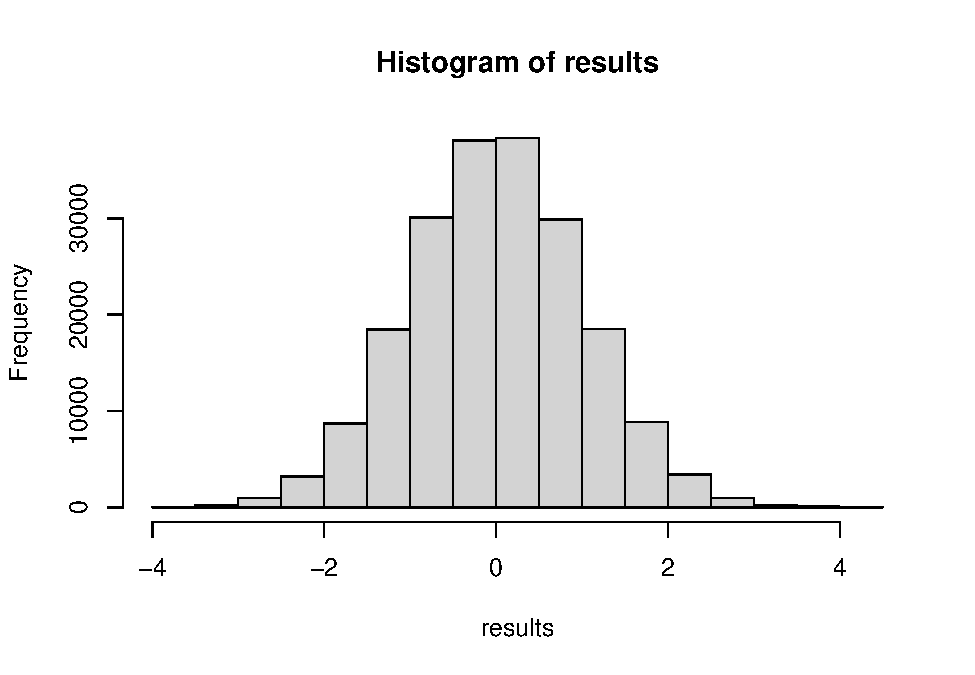
\includegraphics{Aleksi_Patronen_lab1_files/figure-latex/cars-1.pdf}

\begin{Shaded}
\begin{Highlighting}[]
\FunctionTok{set.seed}\NormalTok{(seed)}
\NormalTok{results\_standard }\OtherTok{\textless{}{-}} \FunctionTok{rnorm}\NormalTok{(n)}

\FunctionTok{summary}\NormalTok{(results[,}\DecValTok{1}\NormalTok{]) }\SpecialCharTok{{-}} \FunctionTok{summary}\NormalTok{(results\_standard)}
\end{Highlighting}
\end{Shaded}

\begin{verbatim}
##       Min.    1st Qu.     Median       Mean    3rd Qu.       Max. 
##  0.5259405 -0.0057226 -0.0011024 -0.0007772  0.0045539  0.3785699
\end{verbatim}

Box-Müller and R standard rnorm() dont give exactly the same results.
Slight deviation exist.

b). Make a for loop (or something equivalent) and produce 100 replicate
data sets of the set-up in the earlier part of the exercise. Use the
mean to calculate expectations for each of these, and finally calculate
the standard deviation of the means. Repeat this procedure with n = 100,
1 000 and 10 000. Present a table with n and the standard deviation of
the means. Discuss your result and present the R-code you together with
explaination \# comments.

\begin{Shaded}
\begin{Highlighting}[]
\FunctionTok{plot}\NormalTok{(ns,deviations, }\AttributeTok{type =} \StringTok{"b"}\NormalTok{, }\AttributeTok{xlab =} \StringTok{"number of obs."}\NormalTok{, }\AttributeTok{ylab =} \StringTok{"standard deviations of mean from 100 datasets"}\NormalTok{, }\AttributeTok{col =} \StringTok{"red"}\NormalTok{)}
\end{Highlighting}
\end{Shaded}

\includegraphics{Aleksi_Patronen_lab1_files/figure-latex/unnamed-chunk-1-1.pdf}

It would seem that the standard deviation has an exponential decay in
size. Meaning it is asymptotically standard deviation.

\begin{Shaded}
\begin{Highlighting}[]
\FunctionTok{matrix}\NormalTok{(}\FunctionTok{c}\NormalTok{(ns, deviations), }\AttributeTok{nrow =} \DecValTok{3}\NormalTok{, }\AttributeTok{ncol =} \DecValTok{2}\NormalTok{)}
\end{Highlighting}
\end{Shaded}

\begin{verbatim}
##       [,1]        [,2]
## [1,]   100 0.088828676
## [2,]  1000 0.031657276
## [3,] 10000 0.009486112
\end{verbatim}

\hypertarget{assigment-2}{%
\subsection{Assigment 2}\label{assigment-2}}

a)The purpose of this part is to test the variance reduction properties
of the importance sampling algorithm. The logic behind importance
sampling is to introduce an importance sampling function g(x) into the
integral.

where w(x) are importance weights. Consider the function
h(x)=10exp⁡(-2\textbar x-5\textbar). The first task is to write R code
that implements ordinary Monte Carlo sampling to obtain E(h(X)) where X
\textasciitilde{} Unif(0,10). Use the MC samples to obtain the
expectation, standard deviation and coefficient of variation based on 10
000 samples. Plot X against h(X). \#Add: Compare with the integrate()
function in R.

You will now introduce an importance sampling function g(x)=N⁡(5,1) that
together with f(x)=1⁄10 results in w(x)=(√2π
e\textsuperscript{((x-5)}2⁄2))⁄10. The full integral can be re-written
as

\begin{Shaded}
\begin{Highlighting}[]
\NormalTok{w }\OtherTok{\textless{}{-}} \ControlFlowTok{function}\NormalTok{(x) }\FunctionTok{dunif}\NormalTok{(x, }\DecValTok{0}\NormalTok{, }\DecValTok{10}\NormalTok{)}\SpecialCharTok{/}\FunctionTok{dnorm}\NormalTok{(x, }\AttributeTok{mean=}\DecValTok{5}\NormalTok{, }\AttributeTok{sd=}\DecValTok{1}\NormalTok{) }\CommentTok{\# weights {-}\textgreater{} f/g }
\NormalTok{f }\OtherTok{\textless{}{-}} \ControlFlowTok{function}\NormalTok{(x) }\DecValTok{10}\SpecialCharTok{*}\FunctionTok{exp}\NormalTok{(}\SpecialCharTok{{-}}\DecValTok{2}\SpecialCharTok{*}\FunctionTok{abs}\NormalTok{(x}\DecValTok{{-}5}\NormalTok{)) }\CommentTok{\# f() function (h() in literature) shouln\textquotesingle{}t this be chanced for clarity?}
\NormalTok{X }\OtherTok{\textless{}{-}} \FunctionTok{rnorm}\NormalTok{(}\DecValTok{10000}\NormalTok{,}\AttributeTok{mean=}\DecValTok{5}\NormalTok{,}\AttributeTok{sd=}\DecValTok{1}\NormalTok{) }\CommentTok{\# sampling for X from normal distribution that is: the envelope distr. g()}
\NormalTok{Y }\OtherTok{\textless{}{-}} \FunctionTok{w}\NormalTok{(X)}\SpecialCharTok{*}\FunctionTok{f}\NormalTok{(X) }\CommentTok{\# }


\FunctionTok{hist}\NormalTok{(Y)}
\end{Highlighting}
\end{Shaded}

\includegraphics{Aleksi_Patronen_lab1_files/figure-latex/unnamed-chunk-3-1.pdf}

\begin{Shaded}
\begin{Highlighting}[]
\FunctionTok{summary}\NormalTok{(Y)}
\end{Highlighting}
\end{Shaded}

\begin{verbatim}
##    Min. 1st Qu.  Median    Mean 3rd Qu.    Max. 
##  0.3392  0.4869  0.8095  0.9992  1.3920 27.2343
\end{verbatim}

\begin{Shaded}
\begin{Highlighting}[]
\NormalTok{h }\OtherTok{\textless{}{-}} \ControlFlowTok{function}\NormalTok{(x)\{}\DecValTok{10}\SpecialCharTok{*}\FunctionTok{exp}\NormalTok{(}\SpecialCharTok{{-}}\DecValTok{2}\SpecialCharTok{*}\FunctionTok{abs}\NormalTok{(x}\DecValTok{{-}5}\NormalTok{))\}}

\FunctionTok{plot}\NormalTok{(X, }\FunctionTok{h}\NormalTok{(X))}
\end{Highlighting}
\end{Shaded}

\includegraphics{Aleksi_Patronen_lab1_files/figure-latex/unnamed-chunk-4-1.pdf}
I dont get it.

\begin{enumerate}
\def\labelenumi{\alph{enumi})}
\setcounter{enumi}{1}
\tightlist
\item
  The next task is to transform the IS algorithm into a Sampling
  importance resampling (SIR) algorithm following the lecture notes (and
  course literature) and compare the results with these from a). Use the
  same n and choose m according to recommendations. Discuss the results
  and provide code with explanations.
\end{enumerate}

\begin{Shaded}
\begin{Highlighting}[]
\NormalTok{w }\OtherTok{\textless{}{-}} \ControlFlowTok{function}\NormalTok{(x) }\FunctionTok{f}\NormalTok{(x)}\SpecialCharTok{/}\FunctionTok{dnorm}\NormalTok{(x, }\AttributeTok{mean=}\DecValTok{5}\NormalTok{, }\AttributeTok{sd=}\DecValTok{1}\NormalTok{) }\CommentTok{\# weights {-}\textgreater{} f/g }


\FunctionTok{set.seed}\NormalTok{(}\DecValTok{1234}\NormalTok{)}
\NormalTok{n }\OtherTok{\textless{}{-}} \DecValTok{10000}
\NormalTok{m }\OtherTok{\textless{}{-}} \DecValTok{5000}

\NormalTok{y }\OtherTok{\textless{}{-}} \FunctionTok{rnorm}\NormalTok{(}\AttributeTok{n =}\NormalTok{ m, }\AttributeTok{mean =} \DecValTok{5}\NormalTok{, }\AttributeTok{sd =} \DecValTok{1}\NormalTok{)}
\NormalTok{w }\OtherTok{\textless{}{-}}  \FunctionTok{w}\NormalTok{(y)}
\NormalTok{w }\OtherTok{\textless{}{-}}\NormalTok{ w}\SpecialCharTok{/}\FunctionTok{sum}\NormalTok{(w)}

\NormalTok{x }\OtherTok{\textless{}{-}} \FunctionTok{sample}\NormalTok{(y, }\AttributeTok{replace =} \ConstantTok{TRUE}\NormalTok{, }\AttributeTok{prob =}\NormalTok{ w, }\AttributeTok{size =}\NormalTok{ n)}

\FunctionTok{hist}\NormalTok{(x)}
\end{Highlighting}
\end{Shaded}

\includegraphics{Aleksi_Patronen_lab1_files/figure-latex/unnamed-chunk-5-1.pdf}

Histogram look reasonable approximation of h(x)

\begin{Shaded}
\begin{Highlighting}[]
\FunctionTok{summary}\NormalTok{(x)}
\end{Highlighting}
\end{Shaded}

\begin{verbatim}
##    Min. 1st Qu.  Median    Mean 3rd Qu.    Max. 
##   1.604   4.651   4.993   4.991   5.352   8.196
\end{verbatim}

\end{document}
